%%%%%%%%%%%%%%%%%%%%%%%%%%%%%%%%%%%%%%%%%%%%%%%%%%%%%%%%%%%%%%%%%%%%%%
% LaTeX Example: Project Report
%
% Source: http://www.howtotex.com
%
% Feel free to distribute this example, but please keep the referral
% to howtotex.com
% Date: March 2011 
% 
%%%%%%%%%%%%%%%%%%%%%%%%%%%%%%%%%%%%%%%%%%%%%%%%%%%%%%%%%%%%%%%%%%%%%%
% How to use writeLaTeX: 
%
% You edit the source code here on the left, and the preview on the
% right shows you the result within a few seconds.
%
% Bookmark this page and share the URL with your co-authors. They can
% edit at the same time!
%
% You can upload figures, bibliographies, custom classes and
% styles using the files menu.
%
% If you're new to LaTeX, the wikibook is a great place to start:
% http://en.wikibooks.org/wiki/LaTeX
%
%%%%%%%%%%%%%%%%%%%%%%%%%%%%%%%%%%%%%%%%%%%%%%%%%%%%%%%%%%%%%%%%%%%%%%
% Edit the title below to update the display in My Documents
%\title{Project Report}
%
%%% Preamble






\documentclass[paper=a4, fontsize=11pt]{scrartcl}
\usepackage[T1]{fontenc}  
\usepackage{lmodern}

\usepackage[english]{babel}															% English language/hyphenation
\usepackage[protrusion=true,expansion=true]{microtype}	
\usepackage{amscd}
\usepackage{amsmath}
\usepackage{amssymb}
\usepackage{amsthm}
\usepackage{epsfig}
\usepackage{verbatim}
\usepackage{amsthm}
\pagestyle{empty}
\usepackage{color}
\usepackage{graphicx}	
\usepackage{url}

\setlength{\textheight}{8.5in} \setlength{\topmargin}{0.0in}
\setlength{\headheight}{0.0in} \setlength{\headsep}{0.0in}
\setlength{\leftmargin}{0.5in}	
\setlength{\oddsidemargin}{0.0in}
%\setlength{\parindent}{1pc}
\setlength{\textwidth}{6.5in}
%\linespread{1.6}

%%% Custom sectioning
\usepackage{sectsty}
\allsectionsfont{\centering \normalfont\scshape}


%%% Custom headers/footers (fancyhdr package)
\usepackage{fancyhdr}
\pagestyle{fancyplain}
\fancyhead{}											% No page header
\fancyfoot[L]{}											% Empty 
\fancyfoot[C]{}											% Empty
\fancyfoot[R]{\thepage}									% Page numbering
\renewcommand{\headrulewidth}{0pt}			% Remove header underlines
\renewcommand{\footrulewidth}{0pt}				% Remove footer underlines
\setlength{\headheight}{13.6pt}


%%% Equation and float numbering
\numberwithin{equation}{section}		% Equationnumbering: section.eq#
\numberwithin{figure}{section}			% Figurenumbering: section.fig#
\numberwithin{table}{section}				% Tablenumbering: section.tab#


%%% Maketitle metadata
\newcommand{\horrule}[1]{\rule{\linewidth}{#1}} 	% Horizontal rule

\title{
		%\vspace{-1in} 	
		\usefont{OT1}{cmr}{b}{n}
		\normalsize \textsc{CSci 8551: Project Progress Report} \\ [30pt]
		\horrule{0.5pt} \\[0.4cm]
		\huge Edge detection in images using Ant Colony Optimization Algorithms \\
		\horrule{2pt} \\[0.5cm]
}
\author{
		\normalfont 								\normalsize
        Arjun Varshney\\[-3pt]		\normalsize
        \today
}
\date{}
%%% Begin document
\begin{document}
\maketitle
\section{Things Done So Far}
In this project, we use Ant Colony Optimization (ACO) algorithms \cite{JTWYSX} to detect edges in an image and compare results of various algorithms for a set of images. ACO aims to find the optimal solution to the target problem through a guided search (i.e., the movements of a number of ants) over the image by constructing the pheromone information (matrix of pixel size). To be more specific, suppose totally K ants are applied to find the optimal solution in a space $\chi$ that consists of $M1 \times M2$ nodes, the procedure of ACO can be summarized as follows:

\begin{center}
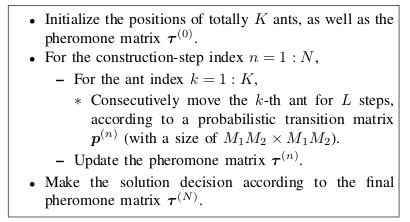
\includegraphics[scale=0.6]{Selection_003.png}
\end{center}

I have implemented the Ant Colony System meta-heuristic for detecting the edges, which is different from other ACO metaheuristics, as it has a local pheromone update too in addition to the pheromone update performed at the end of the construction process (offline pheromone update)\cite{JTWYSX} . The algorithm is broken into four parts, initialization, construction, update and decision process.
 
\subsection{Initialization}
We start with initializing the ants to move on an image for constructing the pheromone matrix. The initialization is done randomly in the \cite{MDKS}, but I have tried various methods (see preliminary results) to find the best position of ants so that the image formation is  better and faster. The pheromone matrix has the information of the edge at each pixel location of the image. The movements of the ants are guided by the local variation of the image's intensity values. This procedure runs for N iterations to construct the pheromone matrix by iteratively performing both the construction and the update process. The decision process is made to find the edge with the updated pheromone matrix values.

\subsection{Construction}
At the n\textsuperscript{th} step, an ant is randomly selected, and this ant is made to move for M steps. This ant moves from the current node to its neighboring node according to a transition probability function. The permissible range of ant's movement is determined by two types of neighborhood (4-connectivity, or 8 connectivity) as shown below. 

\begin{figure}[h!]
\centering
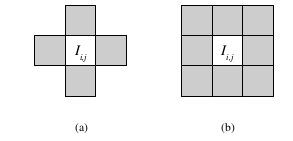
\includegraphics[scale=0.6]{Selection_006.png}
\caption {a) 4-connectivity and b) 8-connectivity neighborhood}
\end{figure}

\subsection{Update}
The update process is a two step process for updating the pheromone matrix.
The first update in done locally after each ant moves a step. Each element of the pheromone matrix associated to that location of the ant is updated to, 

\begin{center}
$\tau_{i,j}^{(n-1)}=\begin{cases}(1 - \rho).\tau_{(i.j)}^{(n-1)}+ \rho.\Delta_{(i,j)}^{(k)} & if (i,j)\ is\ visited\ by\ the\ current\ k^{th}\ ant ;\\ \tau_{i,j}^{(n-1)} & otherwise\end{cases}$
\end{center} where $\tau_{i,j}^{(n-1)}$ is the pheromone value at the (i,j) position of the pheromone matrix, $\rho$ is the evaporation rate and $\Delta_{i,j}^{(k)}$ is determined by the heuristic matrix.

The second update is the global update after all the ants finish one construction step. The pheromone matrix is then globally updated by, 
\begin{center}
$\tau^{n} = ( 1 - \psi). \tau^{(n-1)}+ \psi.\tau^{(0)}$
\end{center} where $\psi$ is the pheromone decay coefficient.

\subsection{Decision}

In this portion, a binary decision is made at each pixel to determine whether it is edge or not, by applying a threshold T on the final pheromone matrix $\tau^{(n)}$. The initial threshold $\tau^{(0)}$ is chosen to be the mean value of the pheromone matrix. The entries of the pheromone matrix is labeled into two class according to the criterion that its value is lower than $\tau^{(0)}$ or larger than $\tau^{(0)}$ . The new threshold is calculated as the average of two mean values of each of above two categories. The above process is repeated till there is no change in the threshold value.

\vspace{1cm}

\section{Preliminary Results}

I ran the Ant Colony System algorithm on the gray scale versions of few of my pencil sketches. The results of the Ant Colony System meta-heuristic are as shown below: 
\begin{itemize}
	\item following results were obtained on placing the ants initially on the random  rows and columns of the image. As expected, initial results were not so good due to bad initial placements of the ants. 
	\begin{figure}[h!]
	\centering     
	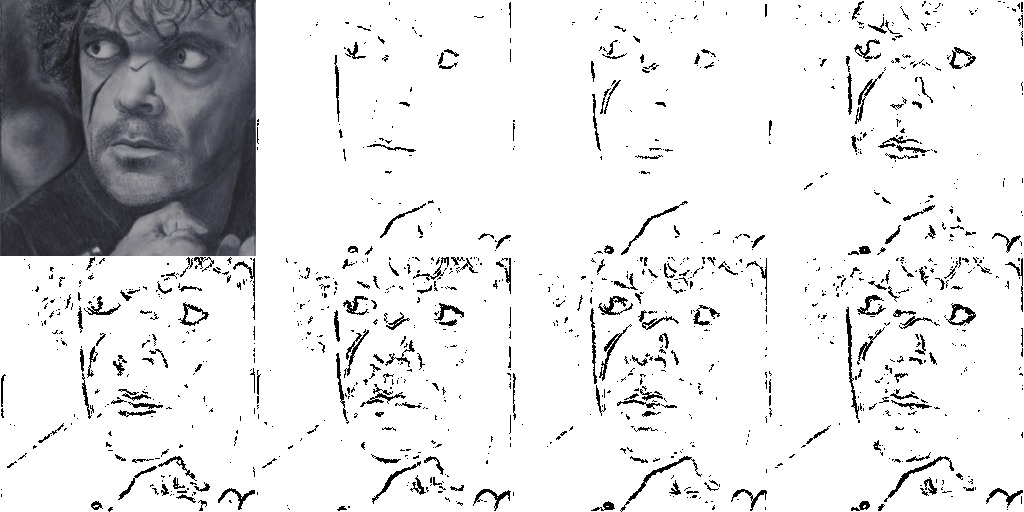
\includegraphics[scale=0.35]{tyrionMixed.jpg}
          \caption{Tyrion : Ants initialized on random rows and columns of the image}
	\end{figure}
	\item following results were obtained on placing the ants initially on the diagonal of the pheromone matrix. The initial result shows clearly that the image edges are detected starting from the diagonal  and the final result was found satisfactory.
    
	\begin{figure}[!h]
	\centering     
	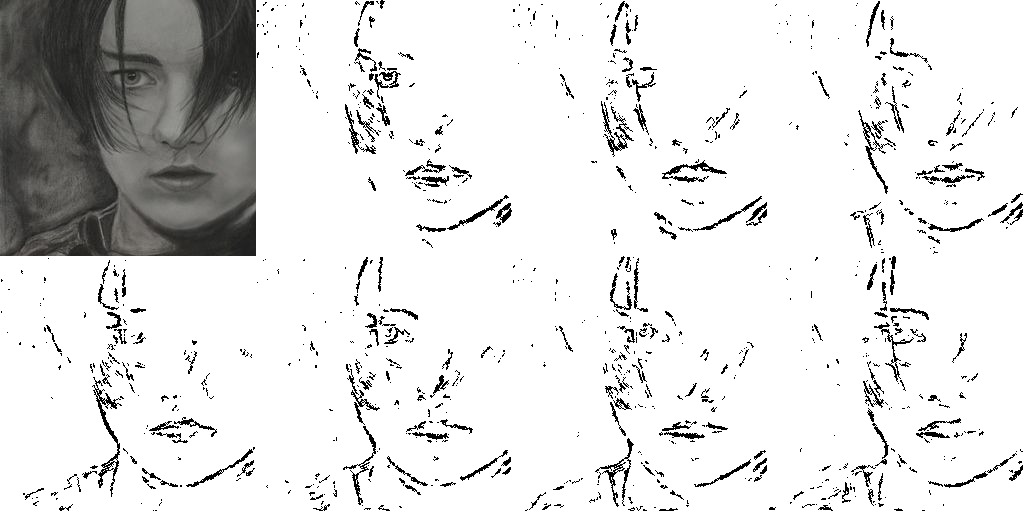
\includegraphics[scale=0.35]{aryaMixed.jpg}
          \caption{Arya : Ants initialized on the diagonal of the image}
	\end{figure}
    \pagebreak
    \item following results were obtained on placing the ants initially on the highest values of the heuristics. The initial results shows clearly that the edges are detected in the first iteration itself. More edges can be identified easily in fewer iterations.
	\begin{figure}[h!]
	\centering     
	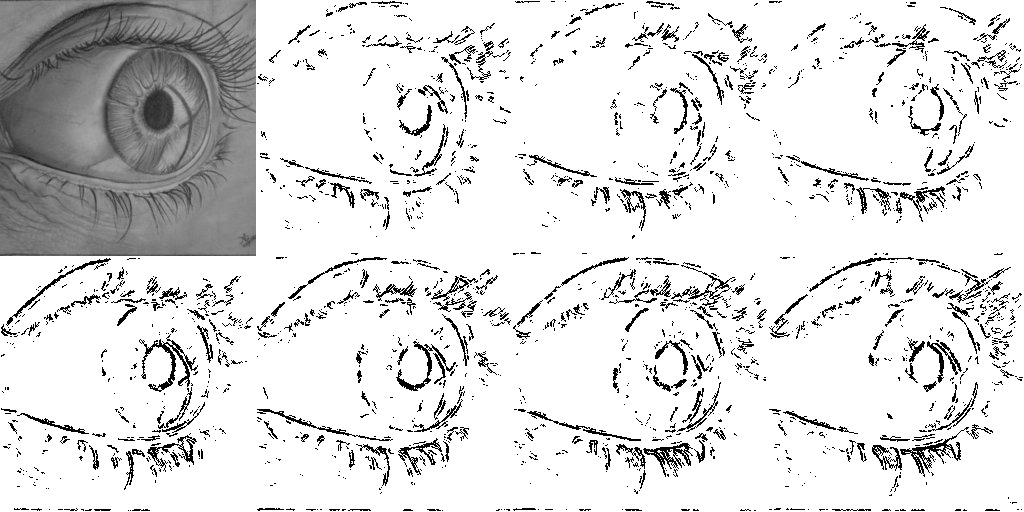
\includegraphics[scale=0.35]{eyemixed.jpg}
          \caption{Arya : Ants initialized on the highest values of the heuristic matrix}
	\end{figure}
\end{itemize}    
\section{Remaining Work}
The plan is to improve the current Ant Colony System Implementation using the initialization of the ants or tweaking some parameters like the threshold as stated in the decision process. Also, Ant System \cite{HNSE} meta-heuristic is yet to be implemented. The comparison of the two algorithms with respect to execution time and the image results, would be the final step of this project. 

\begin{thebibliography}{99}

\bibitem{JTWYSX} Jing Tian, Weiyu Yu, and Shengli Xie,{\textit{An Ant Colony Optimization Algorithm For Image Edge Detection}}, 2008 IEEE Congress on Evolutionary Computation (CEC 2008) 
\bibitem{MDKS} Marco Dorigo and Krzysztof Socha,{\textit{An Introduction to
Ant Colony Optimization}}, April 2006
\bibitem{HNSE} H. Nezamabadi-Pour, S. Saryazdi, and E. Rashedi, {\textit{Edge detection using ant algorithms}} Soft Computing, vol. 10, pp. 623-628, May 2006.
\end{thebibliography}


%%% End document
\end{document}